\documentclass[eso]{bcc}
\usepackage{ifmtarg}% http://ctan.org/pkg/ifmtarg

\newcommand{\citeabnt}[1]{(\textsc{\citeauthor{#1}}, \citeyear{#1})}
\newcommand{\citetabnt}[1]{\citeauthor{#1} (\citeyear{#1})}

\titulo{RELATÓRIO DE ESTÁGIO SUPERVISIONADO OBRIGATÓRIO (ESO)}
\tituloProjeto{As novas possibilidades geradas pela Internet das Coisas para o agronegócio}

\palavrasChave{Internet das Coisas}{Automação}{Agronegócio 4.0.}
\keywords{Internet of Things, Automation, Agrobusiness 4.0.}

\autor{Armstrong Lohãns de Melo Gomes Quintino}{lohansdemelo1108@gmail.com}

\orientador{Assuero Fonseca Ximenes}{Gestão de TI}{UFAPE}
% \orientadorDois{Nome Professor}{Para completar}{UFAPE}


\examinador{Rodrigo Gusmão de Carvalho Rocha}{Engenharia de Software}{UFAPE}
% \examinadorDois{Richard Karp}{Para completar}{UFAPE}
% \examinadorTres{Stephen Cook}{Para completar}{UFAPE}

\dataMesAno{29}{agosto}{2022}

\begin{document}

\selectlanguage{portuguese}

\empresaNome{Universidade Federal do Agreste de Pernambuco}
\empresaArea{Desenvolvimento Mobile}
\empresaPeriodo{01 de agosto de 2019 a 01 de julho de 2020}
\empresaCargaH{20H}
\empresaRemuneracao{R\$ 0,00}
\empresaSupervisorEmail{assuero.ximenes@ufape.edu.br}
\logo{Figuras/UFAPE_logo.png}{0.88}

\capa % With error if not completely filled

% \capaDois

\begin{resumo}
Na atualidade está ocorrendo um aumento na utilização de diversas tecnologias e que, 
pelo aumento do seu uso, tem gerado um grande volume de informações. Esse aumento de 
informação foi devido a utilização da internet e, principalmente, pela utilização de 
diversos dispositivos que se comunicam. Por causa disso e pela inserção dessas tecnologias 
o termo internet das coisas se tornou conhecido em diversas áreas. Desta forma, a proposta 
deste projeto de pesquisa é ressaltar  a  importância  da Internet das Coisas e seus 
impactos econômicos e sociais, por meio de uma revisão bibliográfica e estudos acerca 
da Internet das Coisas aplicada no agronegócio bem como o desenvolvimento de uma aplicação 
simulando uma situação real. E para atingir a finalidade desses impactos diversas bases 
foram utilizadas a fim de embasar o conhecimento sobre a relação entre o paradigma da 
IoT aplicada ao agronegócio, sendo utilizada a pesquisa bibliográfica para este fim. 
Deste modo, o presente trabalho propõe-se a desenvolver uma aplicação simulando uma 
situação real além de compreender o impacto do uso da Internet das Coisas no agronegócio 
com o propósito de auxiliar aos gestores, por meio de informações precisas, o seu processo 
de tomada de decisão.
\end{resumo}

\selectlanguage{english}
\begin{abstract}
Currently, there is an increase in the use of various technologies and, due to 
the increase in their use, they have generated a large volume of information. 
This increase in information was due to the use of the internet and, mainly, 
the use of various devices that communicate. Because of this and the insertion 
of these technologies, the term internet of things has become known in several areas. 
Thus, the purpose of this research project is to emphasize the importance of the 
Internet of Things and its economic and social impacts, through a literature review 
and studies on the Internet of Things applied in agribusiness as well as the development 
of an application simulating a situation real. And to achieve the purpose of these impacts, 
several bases were used in order to base knowledge about the relationship between 
the IoT paradigm applied to agribusiness, using bibliographic research for this purpose. 
In this way, the present work proposes to develop an application simulating a real 
situation in addition to understanding the impact of the use of the Internet of Things 
in agribusiness in order to help managers, through accurate information, your decision-making process.
\end{abstract}
\selectlanguage{portuguese}

% Centralizar titulos
\renewcommand\contentsname{\centerline{Sumário}}
\renewcommand\listfigurename{\centerline{Lista de Figuras}}
% \renewcommand\listtablename{\centerline{Lista de Tabelas}}

\lhead{Sumário}
\tableofcontents

\listoffigures
\addcontentsline{toc}{chapter}{Lista de Figuras}

% \listoftables
% \addcontentsline{toc}{chapter}{Lista de Tabelas}

\newcommand\avisoPIC{
Este trabalho tem como origem um Projeto de Iniciação Científica (PIC), 
onde o mesmo foi realizado na própria Universidade Federal do Agreste de Pernambuco (UFAPE), 
no período que se deu início em 01/08/2019 e concluído no dia 31/07/2020, 
sob orientação do Prof\@. Dr\@. Assuero Fonseca Ximenes, com o título ``As novas 
possibilidades geradas pela Internet das Coisas para o agronegócio'', 
na área da Internet das Coisas, no Curso de Ciência da Computação.
}


\inicio\chapter{Introdução}

\avisoPIC{}

O Brasil, na atualidade, é um dos maiores produtores de alimento do mundo, com potencial para 
ser o maior produtor mundial pelo fato de dispor de vários recursos, principalmente climáticos, 
que favorecem a vasta produção de alimentos.

Além do fator climático, o Brasil apresenta quantidade de água considerável e potencial de 
mais áreas agricultáveis, pois atualmente se utiliza apenas 7,3\% dessas áreas.Associado a isso, 
há mais investimentos em tecnologia, o que difere positivamente nos valores de produção alcançados.

O incremento na utilização de tecnologias se deve ao fato da inserção do termo indústria 4.0, 
surgida na Alemanha, onde, resumidamente, considera-se que a tecnologia digital aplica-se em todos 
os aspectos da sociedade. Desta forma, a agricultura seguiu o termo e se intitula agricultura 4.0, 
pois a mesma se beneficia dos avanços tecnológicos a fim de suprir e melhorar suas necessidades 
de produção na busca de encontrar novas formas de tornar o negócio mais eficiente e competitivo.

Assim, essa nova era agricultura 4.0 trouxe consigo novos questionamentos e, principalmente, 
houve o aumento da preocupação em utilizar o mínimo possível dos recursos naturais e continuar 
produzindo cada vez um volume maior que uma região possa oferecer. Logo, a indústria 4.0 surge 
como uma aliada para otimizar esse sistema e proporcionar essas melhorias.

Diante desse cenário, verifica-se que o Brasil ocupa a posição de 2º maior produtor de alimentos 
do planeta, depois dos Estados Unidos. Uma pesquisa feita em 2017 pela Comissão Brasileira de 
Agricultura de Precisão (CBAP), vinculada ao Ministério da Agricultura, constatou que 67\% das 
propriedades agrícolas do país já utilizam algum tipo de tecnologia na área de gestão do negócio 
e nas atividades de cultivo e colheita da produção. Desta forma, a produção agroindustrial é 
e continua sendo uma válvula de escape fundamental contra a crise econômica que atingiu o Brasil 
nos últimos anos. Em 2015, o setor empregava 19 milhões de pessoas. No ano seguinte, houve aumento 
em cerca de 75 mil novos empregos, segundo dados da Confederação da Agricultura e Pecuária do Brasil 
(CNA) e do Centro de Estudos Avançados em Economia Aplicada (CEPEA).

Ou seja, para possibilitar o agronegócio 4.0 foi necessário conectar coisas com a internet que 
foi chamado de Internet das Coisas (IoT). Desde então, a Internet das Coisas vem se difundindo 
nos mais diferentes ambientes, do meio empresarial ao cotidiano do homem comum estando presente 
nos mais diversos dispositivos que possuem conexão com a internet. Um ponto importante, 
destacado na literatura, é que a IoT tem o potencial de criar um impacto econômico de 
US\$ 2,7 trilhões para US\$ 6,2 trilhões até 2025. Alguns dos usos mais promissores são os 
cuidados com a saúde, as infraestruturas e os serviços do setor público, ajudando a sociedade 
a enfrentar alguns dos seus maiores desafios. (MANYIKA et al., 2013, p. 51).

A partir destes fatos, o objetivo geral deste projeto de pesquisa é apresentar um panorama 
sobre novas possibilidades da IoT dentro do setor do agronegócio e, em específico, 
contextualizar a IoT de forma a levantar, relacionar e fazer uma análise preliminar dessas 
novas possibilidades.Além disso, ressaltar  a  importância  da Internet das Coisas e seus 
impactos econômicos e sociais,  por meio de uma revisão bibliográfica e estudos acerca da 
Internet das Coisas aplicada no agronegócio bem como o desenvolvimento de uma aplicação 
simulando uma situação real.


\section{Objetivos}

\begin{enumerate}
    \item Geral\\
    O objetivo deste projeto é analisar as novas possibilidades geradas pela Internet das Coisas para o agronegócio
    \item Específicos
    \begin{enumerate}
        \item[$-$]  Entender a estrutura da internet das coisas
        \item[$-$] Entender o agronegócio
        \item[$-$] Levantar as novas possibilidades com o uso da Internet das Coisas
        \item[$-$] Relacionar as novas possibilidades pela IoT para o agronegócio 
        \item[$-$] Fazer uma análise preliminar dessas novas possibilidades
        \item[$-$] Desenvolver um aplicativo simulando uma situação real
    \end{enumerate}
\end{enumerate}


% \section{Justificativa}

% Este trabalho se justifica.

% \section{Organização do TCC}

\chapter{Local e Período de Estágio}\label{chap:local}

\avisoPIC{}

Desta forma, o Estágio Supervisionado Obrigatório (ESO) foi realizado originalmente como parte do Projeto de 
Iniciação Científica (PIC) na própria Universidade Federal do Agreste de Pernambuco,
localizada na Rua: Avenida Bom Pastor, s/n.º, bairro: Boa Vista, em Garanhuns, Pernambuco.
As atividades de PIC/ESO foram iniciadas nas datas citadas acima, com carga horária diária 
de 4 horas, totalizando 20 horas semanais, que resultaram em 416 horas ao 
final do PIC/ESO\@.

\chapter{Metodologia}\label{chap:metodologia}
Neste estudo, entende-se que a realidade deve ser interpretada, e não reduzida. Mas para isso 
ocorrer deve-se apreendê-la a partir de sua totalidade. Desta forma será utilizada para esta 
pesquisa a abordagem do tipo exploratória. A pesquisa exploratória permite maior aproximação 
do pesquisador com o objeto investigado, além de possibilitar a coleta de informações sobre 
determinado tema, contribui para aprofundar conceitos ainda preliminares, permitir construir 
as respostas ou refutar as hipóteses levantadas inicialmente pelo investigador. Seu principal 
objetivo é o aprimoramento das ideias e o seu planejamento flexível, permitindo que se considere 
a variedade de aspectos identificados em relação ao fato estudado (GIL, 2008). 
Este tipo de pesquisa visa prover o pesquisador de um maior conhecimento sobre o tema ou 
problema de pesquisa e, por isso, é apropriada para os primeiros estágios da investigação, 
quando a familiaridade, o conhecimento e a compreensão do fenômeno, por parte do pesquisador, 
são geralmente insuficientes ou inexistentes (MATTAR, 1994).

Com a finalidade de responder aos objetivos específicos será utilizada a pesquisa bibliográfica 
que é o levantamento de um determinado tema, processado em bases de dados nacionais e internacionais 
que contêm artigos de revistas, livros, teses e outros documentos (GIL,2008) com a finalidade de 
subsidiar o pesquisador com o conhecimento necessário para analisar as novas possibilidades geradas 
pela Internet das Coisas para o agronegócio.

Após a fase de coleta de dados será possível ser feita a análise de dados, a partir, dessa análise 
documental e relacionar as novas possibilidades ocasionadas pela inserção da internet das coisas.

Posteriormente, com base nos conhecimentos adquiridos, será desenvolvido uma aplicação com a 
utilização de um raspberry que é um minicomputador, semelhante ao PC ou a notebook. A principal 
diferença é que este dispositivo é compacto e possui todos os principais componentes de um 
computador numa pequena placa do tamanho de um cartão de crédito e, com isto permitirá ao 
pesquisador uma aproximação aos dispositivos de IoT atualmente utilizados nas organizações. 
E para simular um ambiente de uma fazenda será utilizado um sensor de umidade de solo que tem 
a função de detectar as variações de umidade no solo, sendo que quando o solo está seco a saída 
do sensor fica em estado alto, e quando úmido em estado baixo.

Para isto, será desenvolvida uma aplicação que coletará esses dados e fornecerá informações para 
a tomada de decisão dos gestores para uma boa gestão do agronegócio.

Inicialmente, a aplicação a ser desenvolvida estará predisposta a dar dados regulares sobre a 
plantação e o clima onde os sensores estão localizados, então, além do sensor de umidade do solo, 
haverá um sensor de temperatura e umidade que incrementará esta coleta de dados, da mesma maneira 
que uma breve consulta sobre o clima atual da região fornecerá informações que serão tratadas 
posteriormente para tomadas de decisão.

\chapter{Fundamentação teórica}\label{chap:fundamentacao}

\section{Internet das Coisas}
O termo Internet of Things (IoT) foi introduzido em 1999 por Kevin Ashton, 
co-fundador do Auto-ID Center do Massachusetts Institute of Technology (MIT). 
Segundo Ashton (2009), a ideia original da IoT previa a conexão de todos os objetos 
físicos à Internet, com capacidade de capturar informações por meio de identificação 
por radiofrequência (RFID) e tecnologias de sensoriamento –as quais os permitiriam observar, 
identificar e compreender o mundo independentemente das pessoas e suas limitações de tempo, 
atenção e precisão.

Em 2005, a União Internacional de Telecomunicações (UIT) previu que a possibilidade de 
identificação única de itens, associada a tecnologias de sensores e a capacidade de interagir 
com o ambiente criaria uma Internet das Coisas (ITU-T, 2016). 

De acordo com Davis (2017) ocorreu quatro estágios de evolução da Internet – Web 1.0, voltada 
para a conexão e obtenção de informações na Rede; Web 2.0 ou Web Social, caracterizada pela 
preocupação com a experiência do usuário e a colaboração por meio das redes sociais; 
Web 3.0 ou Web Semântica, com esforços concentrados na atribuição de significado e contexto 
às informações; e o estágio atual, a Web Ubíqua, constituída pela Internet das Coisas (IoT), 
fundamentada pela conectividade e interatividade entre pessoas, informações, processos e objetos, 
por meio de tecnologias que possibilitam acesso à rede por qualquer pessoa, de qualquer lugar, 
a qualquer tempo, utilizando quaisquer dispositivos, incluindo equipamentos multifuncionais com 
sensores inteligentes, tais como eletrodomésticos, automóveis, roupas, etc., a partir de 
aplicações que se adaptam dinamicamente às necessidades dos usuários (DAVIS, 2017). 

Por causa disto, o mundo físico está se tornando um grande ecossistema de informação em que 
os objetos tanto podem sentir o ambiente como se comunicar independentemente de intervenções humanas. 
Assim, esses objetos tornam-se participantes ativos nos processos de negócio e passam a ser 
reconhecidos e identificados em ambientes inteligentes, que geram informações na Internet, 
promovendo sua funcionalidade adaptativa e responsiva (WEBER, 2015).

Desta forma, a IoT afeta a humanidade em diferentes escalas e envolve desde nanochips implantados 
em seres vivos a objetos de uso comum interconectados, equipados com sensores e identificados 
e que capazes de trocar informações com as pessoas ou com o ambiente. Em face disto, cidades 
estão sendo projetadas de maneira totalmente conectada e automatizada (as chamadas smart cities 
ou cidades inteligentes). As formas de manifestação da IoT são heterogêneas, incluindo dispositivos 
de múltiplos propósitos (celulares, tablets, relógios e óculos inteligentes) e dispositivos 
especializados (sensores de temperatura, dispositivos ativos e passivos, etc.), suportados por 
uma variedade de plataformas de software e hardware. Por isso, o desafio de projetar espaços na 
IoT é contemplar os diferentes níveis de granularidade de forma transparente, garantindo a 
interoperabilidade.

Em face dessas mudanças, as inovações que surgem no âmbito da IoT ampliam o potencial humano 
em diversas áreas tais como planejamento urbano (cidades, edifícios e transito inteligentes), 
meio ambiente (energia, água), indústria, comércio, turismo, educação, saúde, trabalho, 
segurança, programas sociais, governo e agronegócio, promovendo soluções capazes de 
desenvolvimento econômico, sustentabilidade e qualidade de vida.

\section{Gestão de agronegócios}
De acordo com Saab, Neves e Cláudio (2009), o termo agronegócio (agribusiness em inglês) teve 
sua origem na Universidade de Harvard e propõe uma visão sistêmica do funcionamento das atividades 
ligadas à agropecuária.

Ainda conforme esses autores, o agronegócio é formado por vários sistemas agroindustriais  
associados  aos  principais  produtos,  incluindo  todas  as  fases  de  produção até o 
consumidor final. Segundo Reis (2017),os sistemas agroindustriais podem ser divididos em 
três segmentos: (i) setor a montante – responsável por insumos e por bens de capital para a agropecuária; 
(ii) agropecuária – responsável pela produção dos produtos; e 
(iii) setor a jusante – responsável pela industrialização e distribuição.

No atual contexto, o agronegócio, em termos mundiais, demonstra ser muito importante tanto 
econômica quanto socialmente. Conforme a Food And Agriculture Organization Of The United Nations (FAO), 
cerca de 1,02 bilhões de pessoas sofrem com a fome crônica no mundo atualmente (FAO, 2018). 
Essa organização ainda destaca que um dos grandes desafios do agronegócio no futuro será o de 
alimentar uma população projetada de 9,2 bilhões de pessoas em 2050.

A FAO (2018) ainda destaca que os principais desafios da produção do agronegócio poderiam ser 
divididos em: (a) mudanças nos hábitos alimentares da população; (b) mudanças climáticas; 
(c) desenvolvimento da bioenergia; e (d) escassez dos recursos naturais. Apesar dos desafios 
inerentes ao agronegócio, algumas informações ao redor do mundo indicam estatísticas favoráveis 
e que podem ser exploradas pelos gestores nas diversas cadeias agroindustriais.

Vale salientar que essas estatísticas estão relacionadas a países em desenvolvimento, 
tais como o Brasil, a Índia, a Rússia e a China (FULLER et al., 2016) e pode-se dizer que a 
posição do Brasil no que tange ao agronegócio, em geral, é muito favorável além de que o 
agronegócio é muito importante para a economia brasileira. Nesse sentido, Lourenço (2016) 
afirma que o agronegócio brasileiro é um dos principais setores da economia nacional, conseguindo 
atingir posição  de  destaque  mesmo  em  condições  desiguais  de  competição.

Considerando  todo  o  contexto  apresentado,  parece  importante  que  os  gestores  das 
organizações  relacionadas  ao  agronegócio  tenham  a  capacidade  de  gerir seus negócios 
de forma adequada, obtendo os benefícios dessa provável expansão brasileira, assim como 
minimizando os riscos de suas atividades. Pode-se dizer que a gestão dessas organizações 
se situa atualmente em um contexto de aumento da competitividade nos vários segmentos do 
agronegócio em nível mundial (REARDON et al., 2015). Nesse sentido, Fischer et al (2018) destacam 
que  a  maioria  dos  consumidores  ao  redor  do  mundo  pode  escolher  entre uma grande 
variedade de produtos relacionados às cadeias agroindustriais, sendo que milhares de novos 
produtos são inseridos no mercado todos os anos, fazendo com que a competitividade dos negócios 
se torne cada vez mais forte.

\section{A tecnologia e o agronegócio}
Na atualidade, percebe-se  que diversos setores que envolvem a agricultura brasileira tem utilizado 
cada vez mais tecnologias na busca do incremento de mais produtividade. Conforme relatório da 
empresa DATUM (2016), muitas empresas de Tecnologia da Informação geraram confiabilidade na realização 
de projetos direcionados à melhoria dos sistemas de produção agrícola, pois com o auxílio tecnológico 
e a evolução da economia, a produção agrícola ficou mais prática e ágil.

Segundo o ministério da agricultura, pecuária e abastecimento, o Brasil é um dos principais 
fornecedores agrícolas do mundo e o agronegócio representa 1/3 do PIB brasileiro, tendo grande 
relevância para a economia do país (MAPA, 2017).

Desta forma, a tecnologia da informação pode agregar valor a esse mercado criando soluções 
inteligentes para gerar eficácia e melhoria dos processos internos, assertividade no controle da 
produção e agilidade na comercialização, além de evitar desperdício de recursos naturais, como 
por exemplo, o gerenciamento da irrigação no plantio por meio de dispositivos que monitoram o 
volume de água (DATUM, 2016).

Nesse contexto, Cócaro e Jesus (2018) afirmam que como ocorreu no setor urbano, às novas 
tecnologias da informação estão sendo aplicadas ao agronegócio e integrando-se velozmente entre si, 
como por exemplo, as tecnologias de informação com as tecnologias de controle; as tecnologias de 
monitoramento com as tecnologias de telecomunicações que estão fundindo-se rapidamente e aumentando 
os recursos e resultados.

Deste modo é evidente que o setor de tecnologia da informação surge como uma ferramenta de 
desenvolvimento econômico, por possuir resultados confiáveis com rapidez e eficiência que 
indica maior produção e, por consequência, maior retorno financeiro. Assim, a tecnologia da 
informação no agronegócio é vista como um diferencial econômico, uma vez que consegue proporcionar 
vantagens competitivas (IAGRAN, 2015).

De acordo Mendes (2015), o agronegócio vem se tornando importante e influente na economia 
brasileira, por se tratar de algo dinâmico e competitivo. Mas essas características são devidas 
ao fato de estarem correlacionadas com a tecnologia da informação e suas ferramentas de apoio que, 
por meio da utilização de softwares específicos em cada área está sendo capaz de precaver erros 
e enfatizar acertos, de forma a viabilizar e agilizar o processo final de entrega.

Assim, a manutenção e o fortalecimento da capacidade de gerar inovações representa um desafio 
que se impõe para o futuro das organizações. A geração de inovações tecnológicas para complexos 
sistemas de produção agropecuária e a crescente atenção às dimensões econômica, ambiental e 
social exigirão novas estratégias de pesquisa e transferência de tecnologia, além da ampliação 
de arranjos e parcerias com entidades públicas e privadas no Brasil e no exterior. 
Entre as diversas estratégias para enfrentar esses desafios, destaca-se a utilização 
intensa de tecnologias de informação e comunicação (KALSING, 2015).

Neste sentido, são realizadas pesquisas e congressos para constatar a viabilidades e 
assertividades das tecnologias nas empresas e dentro do agronegócio. Na busca de mapear 
esta cadeia e verificar os pontos positivos e negativos, a internet é vista como uma importante 
ferramenta capaz de permitir avanço e crescimento ao agronegócio, por oferecer recursos que 
auxiliam no aumento comercial do mercado. Por meio de instrumentação avançada, agropecuária de 
precisão, bioinformática, data-mining, geotecnologias, modelagem, plataformas web de 
transferência tecnológica, entre outras tecnologias, são disponibilizados instrumentos e 
vertentes de inovação para o agronegócio (KALSING, 2015).

De acordo com TACCHI (2017), dentre as ferramentas para gestão administrativa a Internet 
auxilia na distribuição da importância do uso das tecnologias na vida rural. Hoje os portais 
agropecuários disponibilizam informações sobre as produções, sobre os bancos de dados, sobre 
os softwares utilizados, e fazem a ligação que leva a aquisição dessas ferramentas que permite 
a troca de informação. Segundo o autor, diante da volume de conteúdos é necessário saber gerir 
a informação e o conhecimento em favor da inovação, da sustentabilidade e da vantagem competitiva. 
Com auxílio da tecnologia, pode-se utilizar o meio mais objetivo, rápido e eficaz de modo a 
disponibilizar informação para gerar conhecimento, oportunidades e negócios. 

Porém, toda essa tecnologia deve ser analisada, estudada e introduzida com cuidado, 
pois segundo Noronha e Peres (2015), o valor final das decisões tomadas de forma incorreta, 
é muito maior que o aumento da tecnologia e da competitividade no mercado. 
O avanço da internet tem crescido, auxiliando na quebra de barreiras, encurtando distâncias e 
por fim tem aproximado o produtor rural e o agro negociador de toda essa tecnologia de forma mais rápida.

\chapter{Atividades Desenvolvidas}\label{chap:atividades}

\avisoPIC{}

\section{Resultados esperados}
Como resultados, pretende-se identificar uma solução de baixo custo voltada para o agronegócio 
com aplicações da IoT e desenvolver um software capaz de ajudar na tomada de decisão do agricultor, 
trazendo para perto as tendências da Indústria 4.0. Dessa forma, pode-se estudar e quantificar os 
impactos positivos dessas medidas adotadas concedidas pela Internet das Coisas aplicada neste meio.

\section{Ambiente de Desenvolvimento}
Desta forma, o software desenvolvido foi para a plataforma mobile, visto que um dispositivo 
celular é compacto e, em sua maioria, mais barato que um computador, esta foi uma escolha 
tomada visando a fácil expansão e utilização da ferramenta desenvolvida.

O primeiro passo tomado foi configurar o ambiente onde a planta será observada para que o 
Raspberry e seus sensores obtenham os  dados necessários, estes então serão enviados para a 
nuvem (foi configurado uma instância no Firebase $-$ BaaS do Google), onde fica facilmente acessível 
para os dispositivos inteligentes se comunicarem, promovendo então uma experiência em tempo real, 
onde qualquer alteração na planta surtirá em informações atualizadas no app, facilitando a vida 
do agricultor.

\section{Aplicativo}
Esta é a tela inicial do aplicativo, onde o usuário poderá se cadastrar ou fazer login com 
os dados válidos (Figura I). Suas informações estarão guardadas junto dos dados da planta.

\begin{figure}[htbp]
\centerline{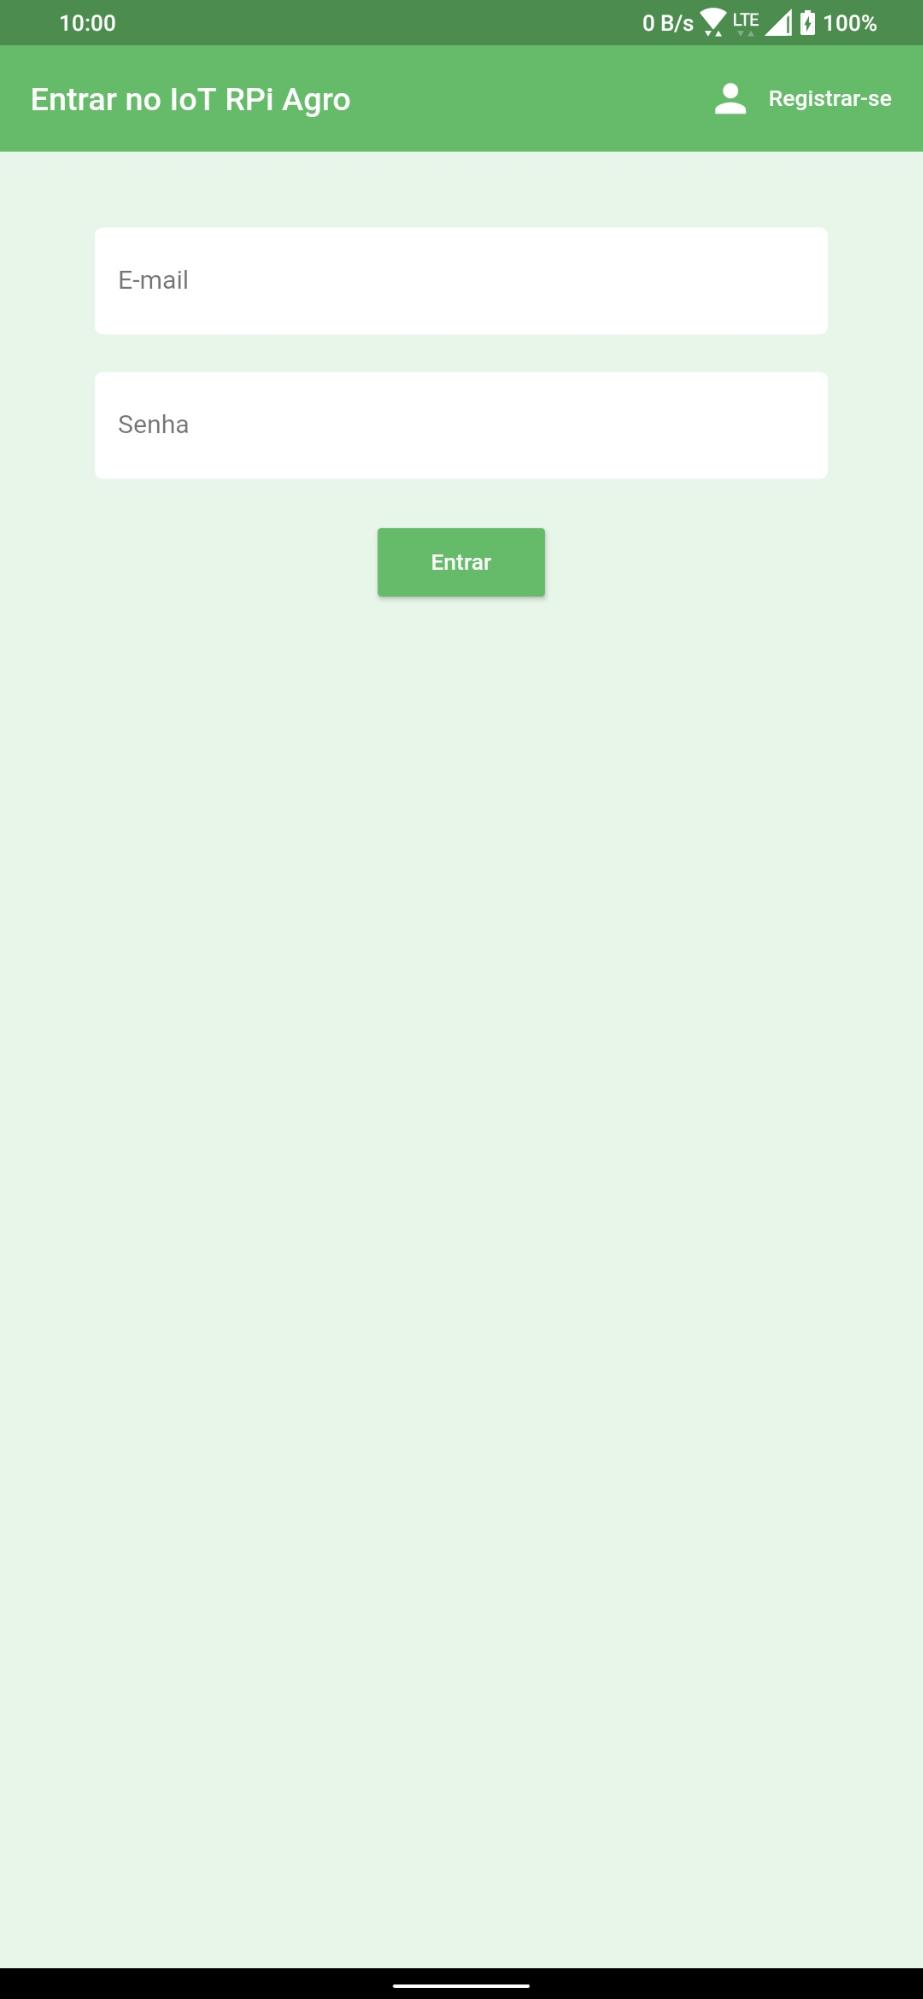
\includegraphics[scale=.25]{Figuras/figura-i.jpg}}
\caption{Figura I}\label{fig-i}
\end{figure}

Na Figura II, após ter entrado com seus dados, é possível verificar que o usuário já possui 
acesso às informações relevantes, além da sugestão de tomada de decisão sobre a irrigação manual da planta.


\begin{figure}[htbp]
\centerline{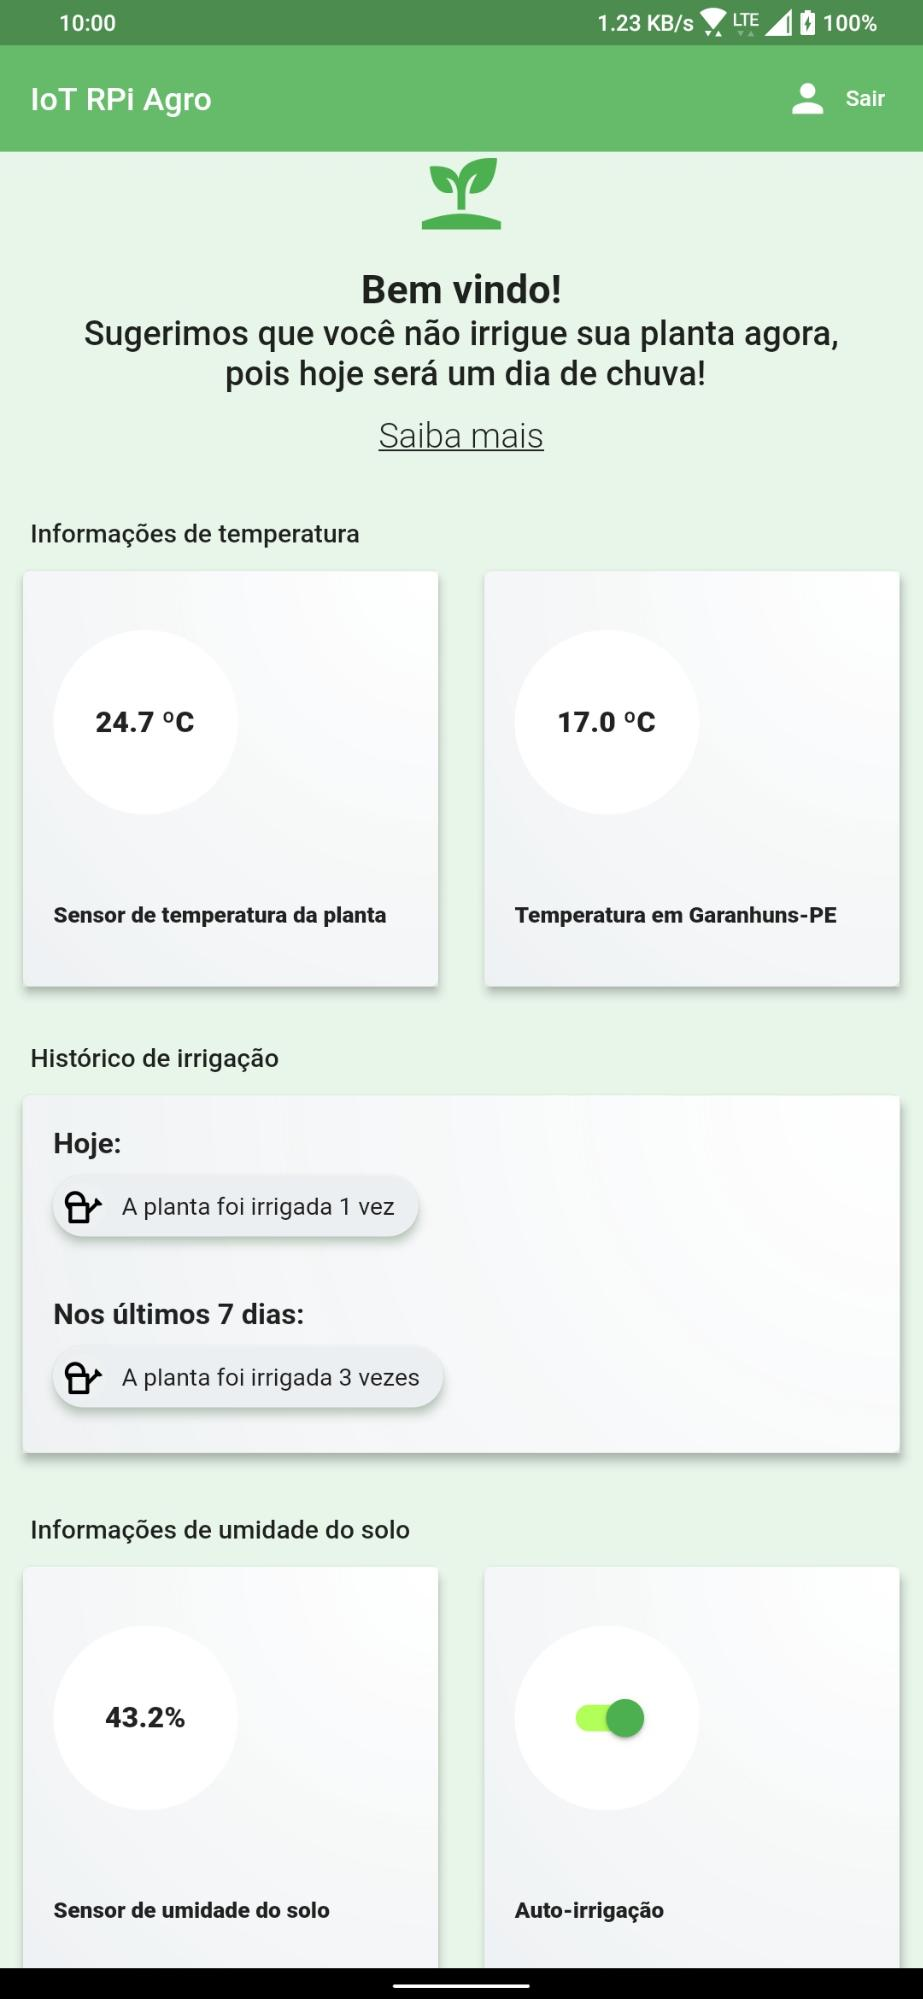
\includegraphics[scale=.25]{Figuras/figura-ii.jpg}}
\caption{Figura II}\label{fig-ii}
\end{figure}

Ao tocar em alguns dos tiles (quadrado com informação) o usuário é redirecionado para outra tela 
contendo informações mais detalhadas.

Nestes dois exemplos ao lado, nas figuras III e IV, é possível observar o detalhamento do sensor 
de temperatura e umidade da planta, e do sensor de umidade do solo, respectivamente.

\begin{figure}[htbp]
\centerline{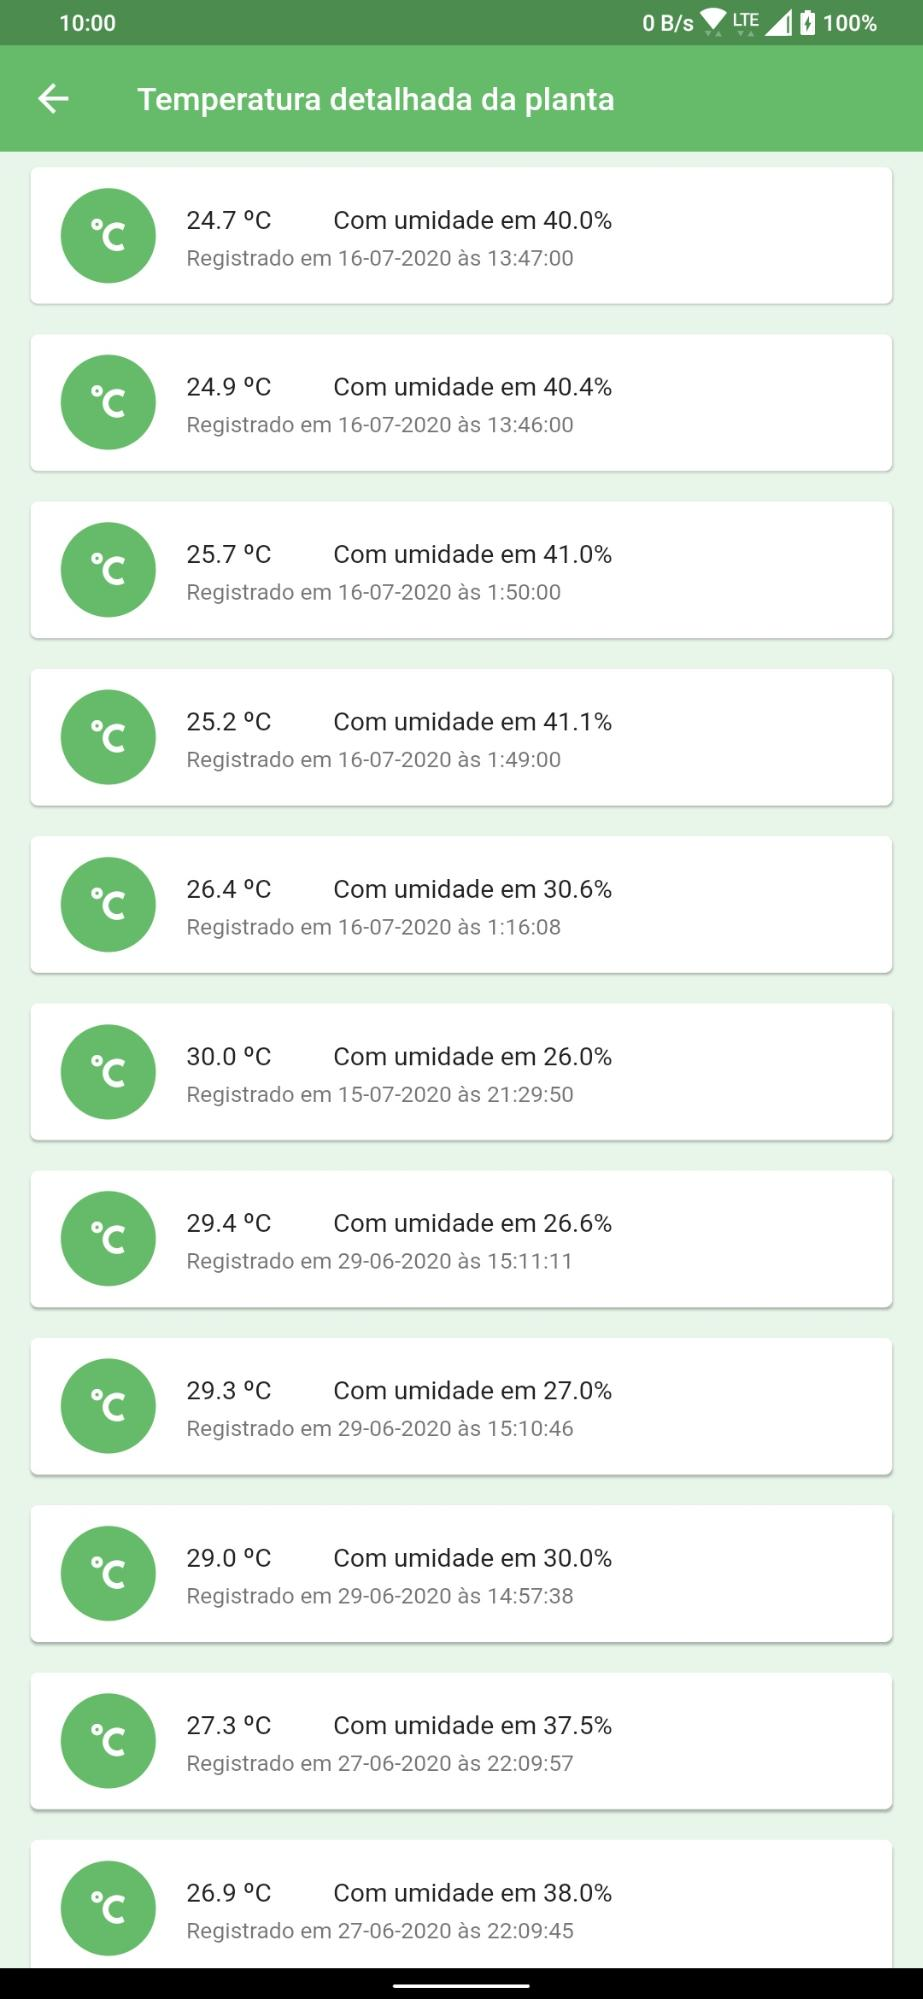
\includegraphics[scale=.25]{Figuras/figura-iii.jpg}}
\caption{Figura III}\label{fig-iii}
\end{figure}

\begin{figure}[htbp]
\centerline{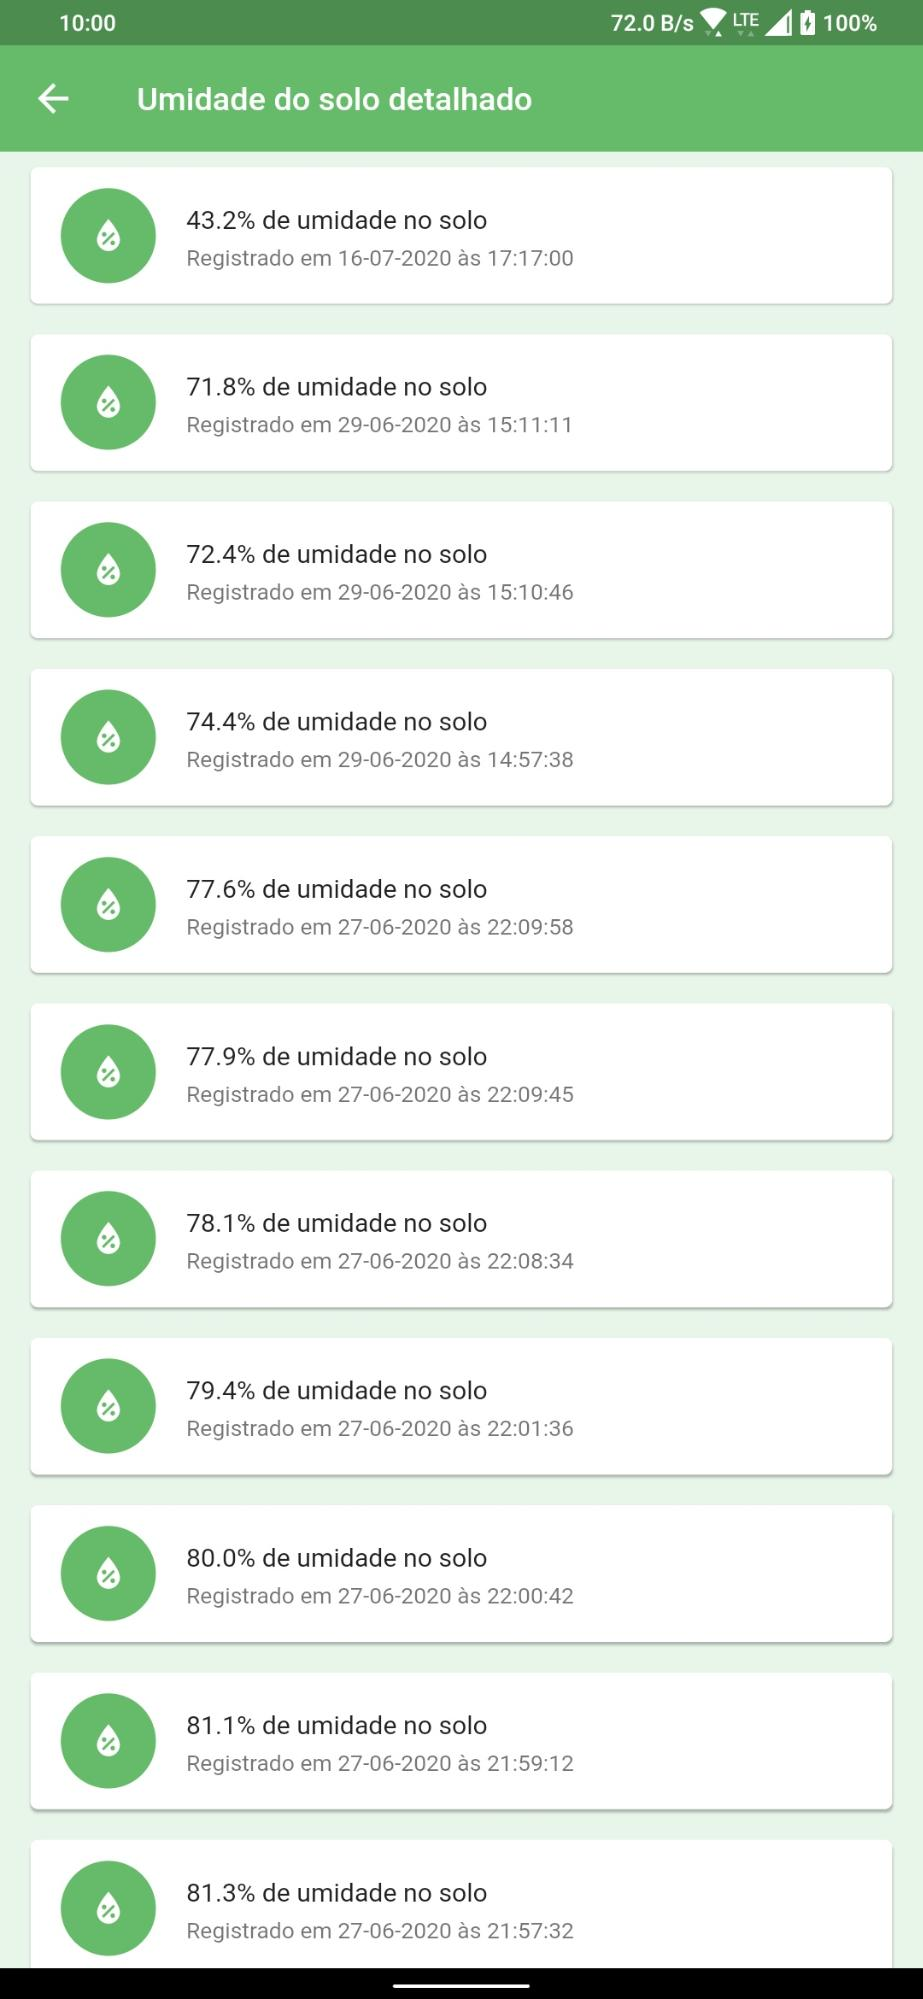
\includegraphics[scale=.25]{Figuras/figura-iv.jpg}}
\caption{Figura IV}\label{fig-iv}
\end{figure}

Os dados são dinamicamente recuperados da nuvem, e qualquer informação gerada pelo sensores será 
atualizada em tempo real no aplicativo.

Além dos dados gerados pela planta, o aplicativo utiliza uma API para obter a previsão do tempo 
e as condições climáticas da região no momento em que o app é aberto, de forma rápida, uma API 
nada mais é que um conjunto de rotinas e padrões de programação para acesso a um aplicativo de 
software ou plataforma baseado na Web para a obtenção de dados específicos.

Na Figura V é possível notar os dados de previsão do tempo para  a localização do usuário, 
da mesma maneira, estão presentes informações relevantes, como a porcentagem de umidade do 
solo atual,  para que o usuário entenda o processo de tomada de decisão.

\begin{figure}[htbp]
\centerline{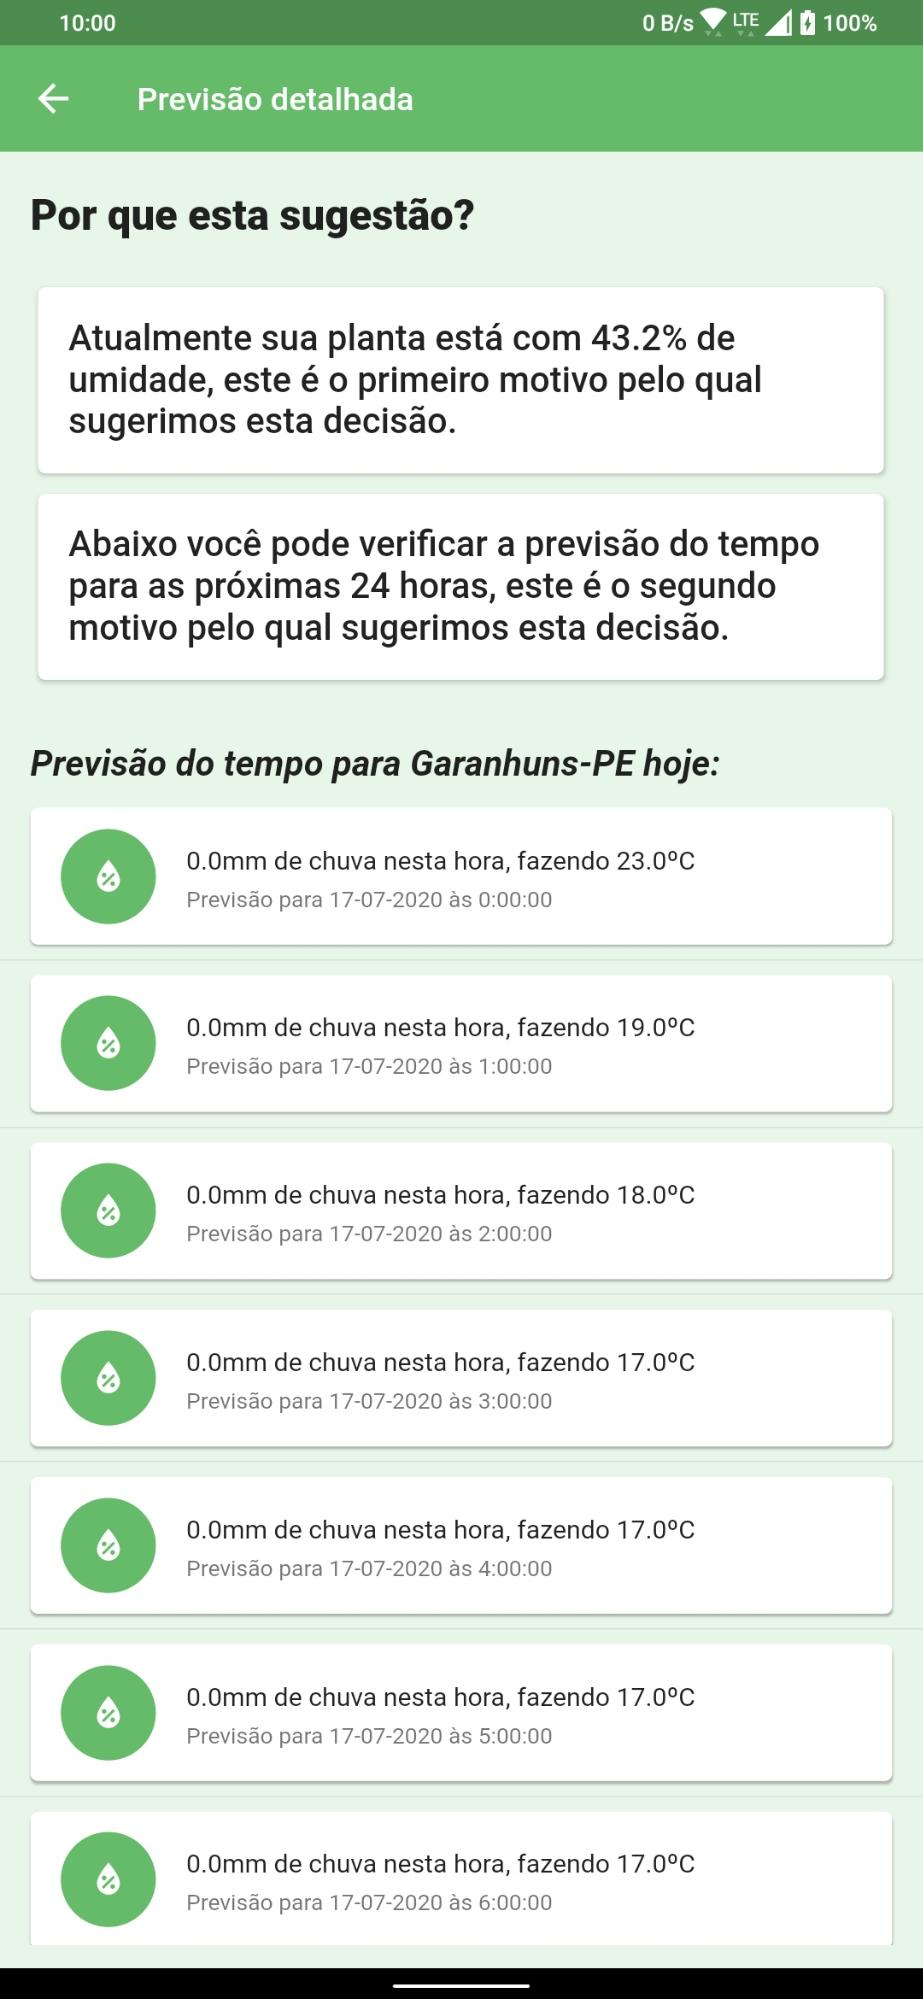
\includegraphics[scale=.25]{Figuras/figura-v.jpg}}
\caption{Figura V}\label{fig-v}
\end{figure}

Na Figura VI, a tela de informações da irrigação automática é mostrada ao usuário quando ele clica 
em seu respectivo tile, onde um log evidencia a hora de registro e a situação em que a opção estava 
no momento, fornecendo informações precisas ao usuário. Estas informações complementam-se com a da 
tela inicial, na área de “Histórico de irrigação”, onde é informado a quantidade de vezes que a 
irrigação foi ativada para a planta, por dia e nos últimos sete dias (observar na figura II).

\begin{figure}[htbp]
\centerline{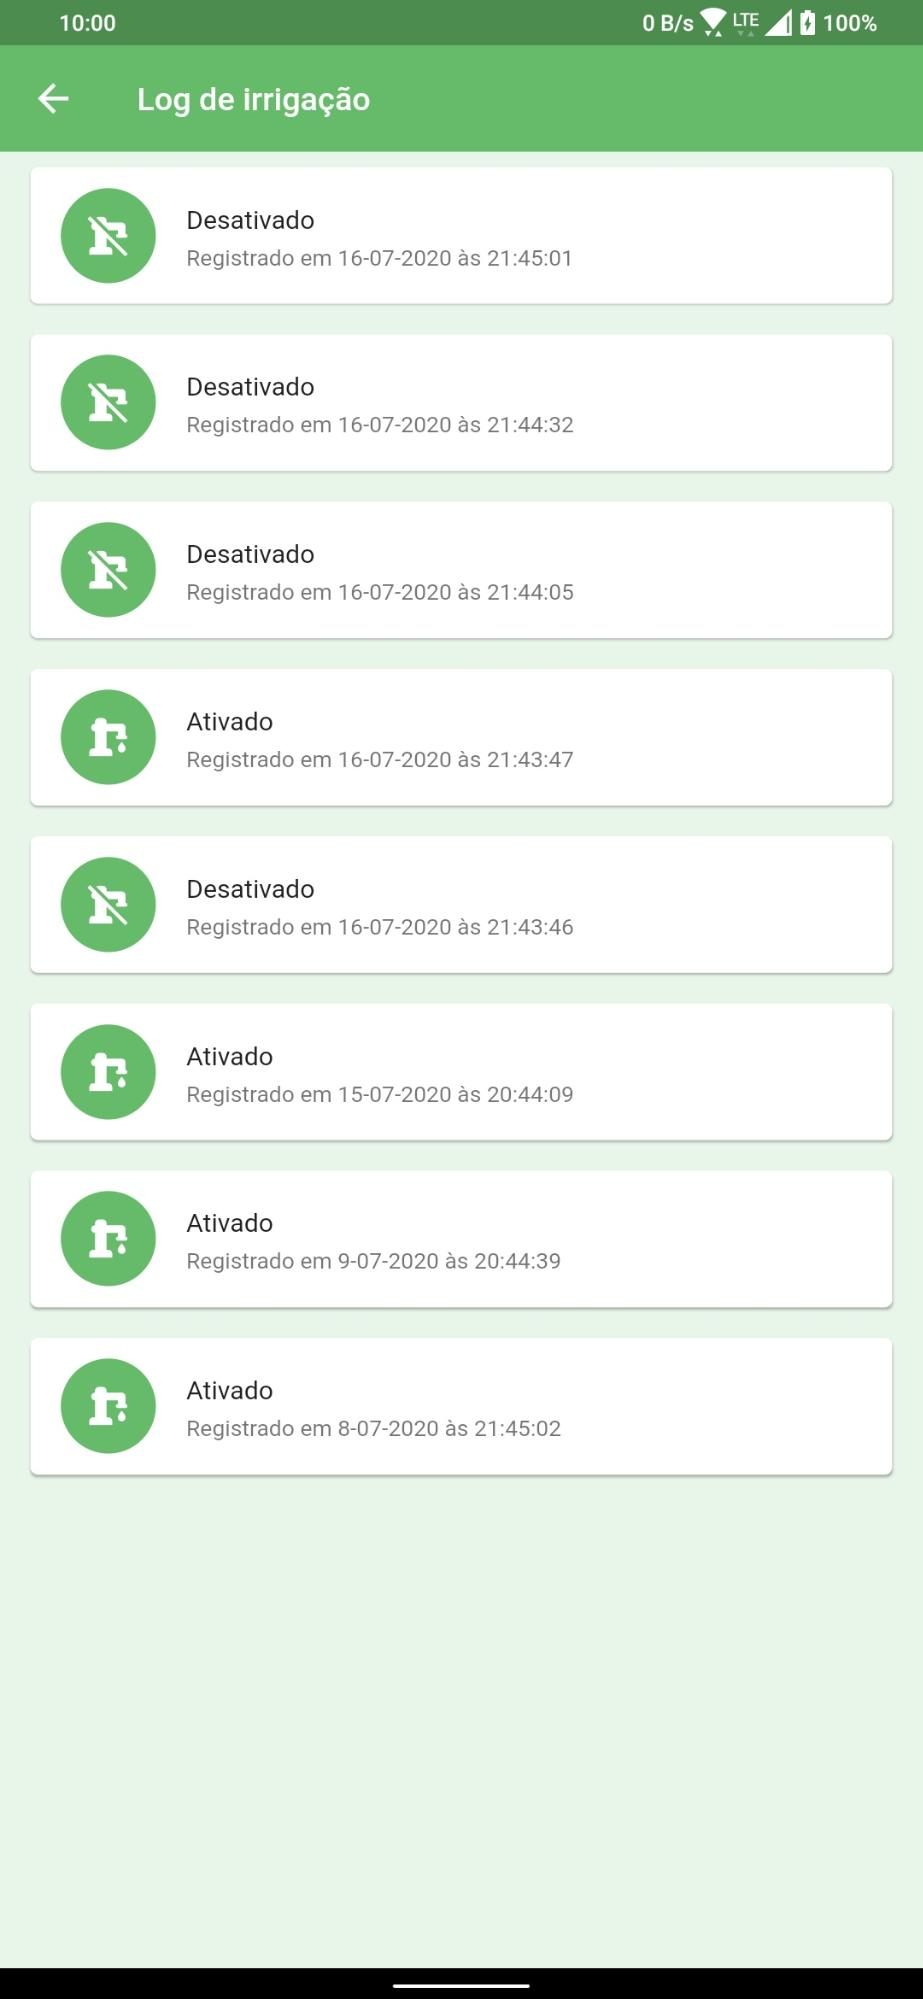
\includegraphics[scale=.25]{Figuras/figura-vi.jpg}}
\caption{Figura VI}\label{fig-vi}
\end{figure}

Nas figuras abaixo, estão presentes as informações sucintas que são mostradas ao usuário dependendo 
da condição metereológica do dia e da condição de temperatura e umidade da planta. Gerando uma 
decisão que pode ser acatada pelo usuário para auxiliar em suas escolhas.	O caso da Figura VII 
acontece quando a planta oferece um bom nível de umidade do solo, e as condições climáticas são 
favoráveis a mantê-la não irrigada pelas próximas horas.	O caso da Figura VIII acontece quando a 
planta está em um nível de umidade do solo moderado, mas a previsão é que chova em pouco tempo, 
fazendo com que seja desnecessária a irrigação manual, assim, economizando água. E por fim, o caso 
da Figura IX acontece quando a planta oferece um baixo nível de umidade do solo, e as condições 
climáticas não são favoráveis a mantê-la sem água pelas próximas horas.

\begin{figure}[htbp]
\centerline{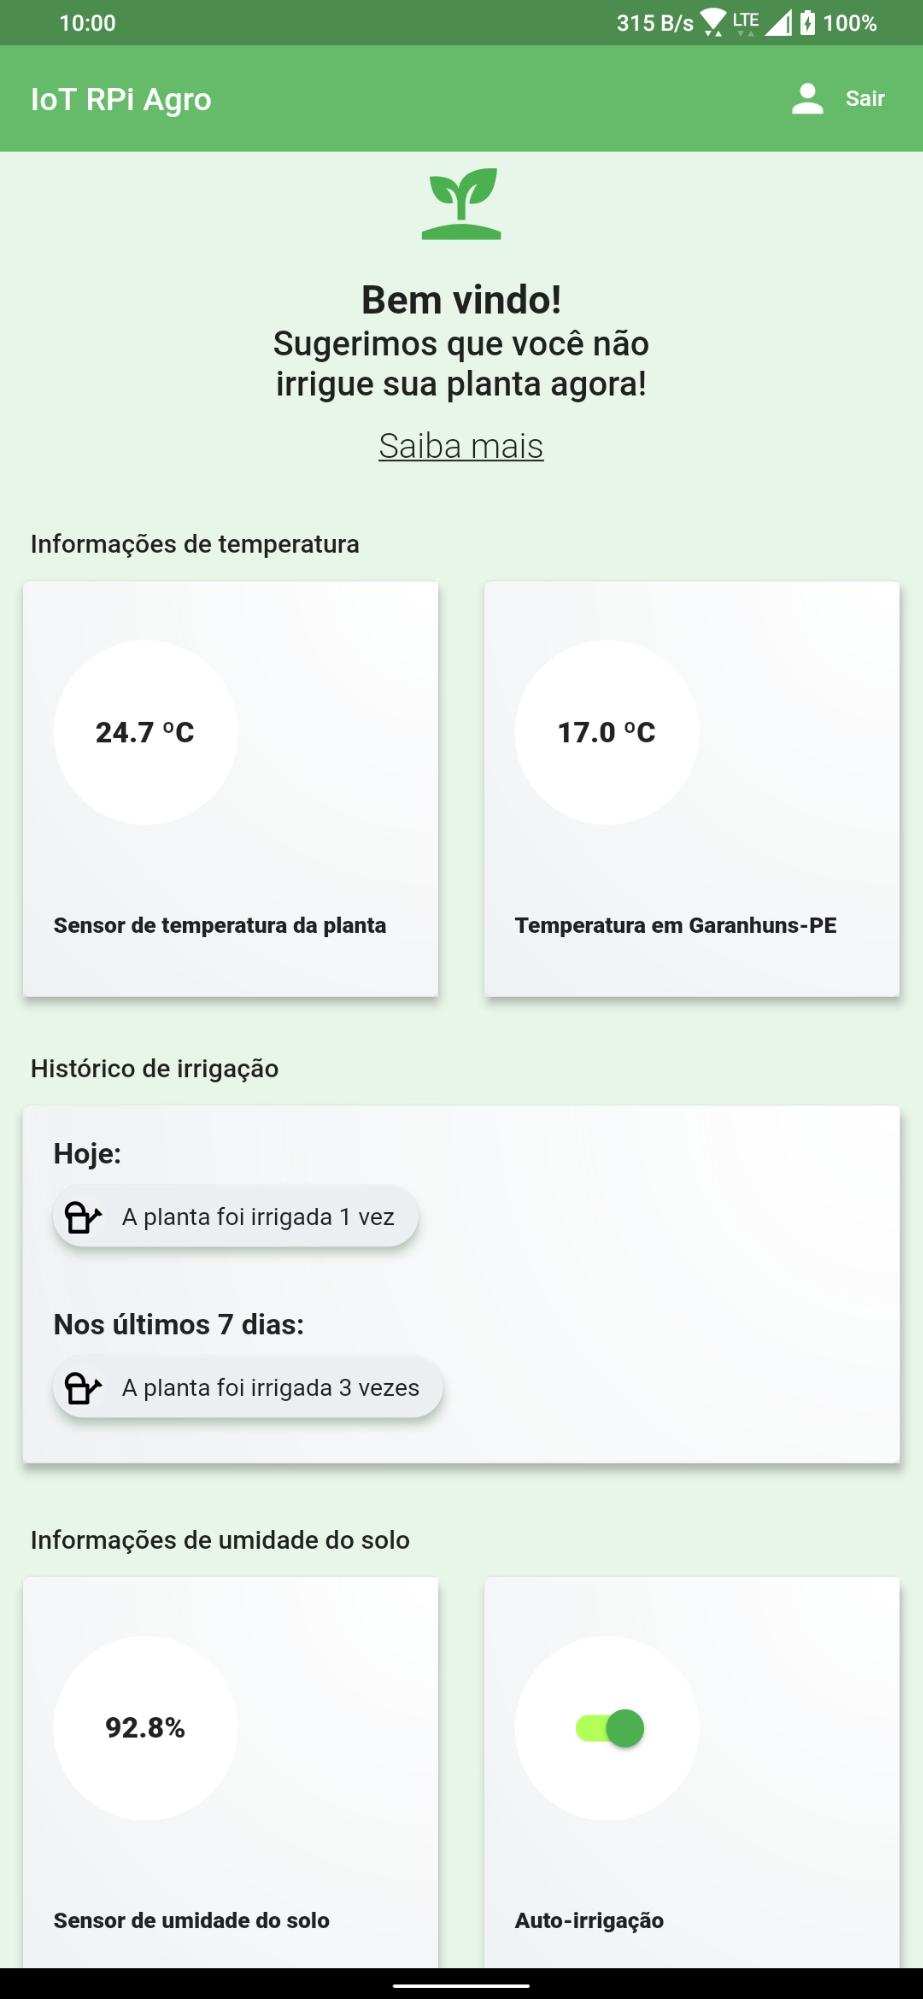
\includegraphics[scale=.25]{Figuras/figura-vii.jpg}}
\caption{Figura VII}\label{fig-vii}
\end{figure}

\begin{figure}[htbp]
\centerline{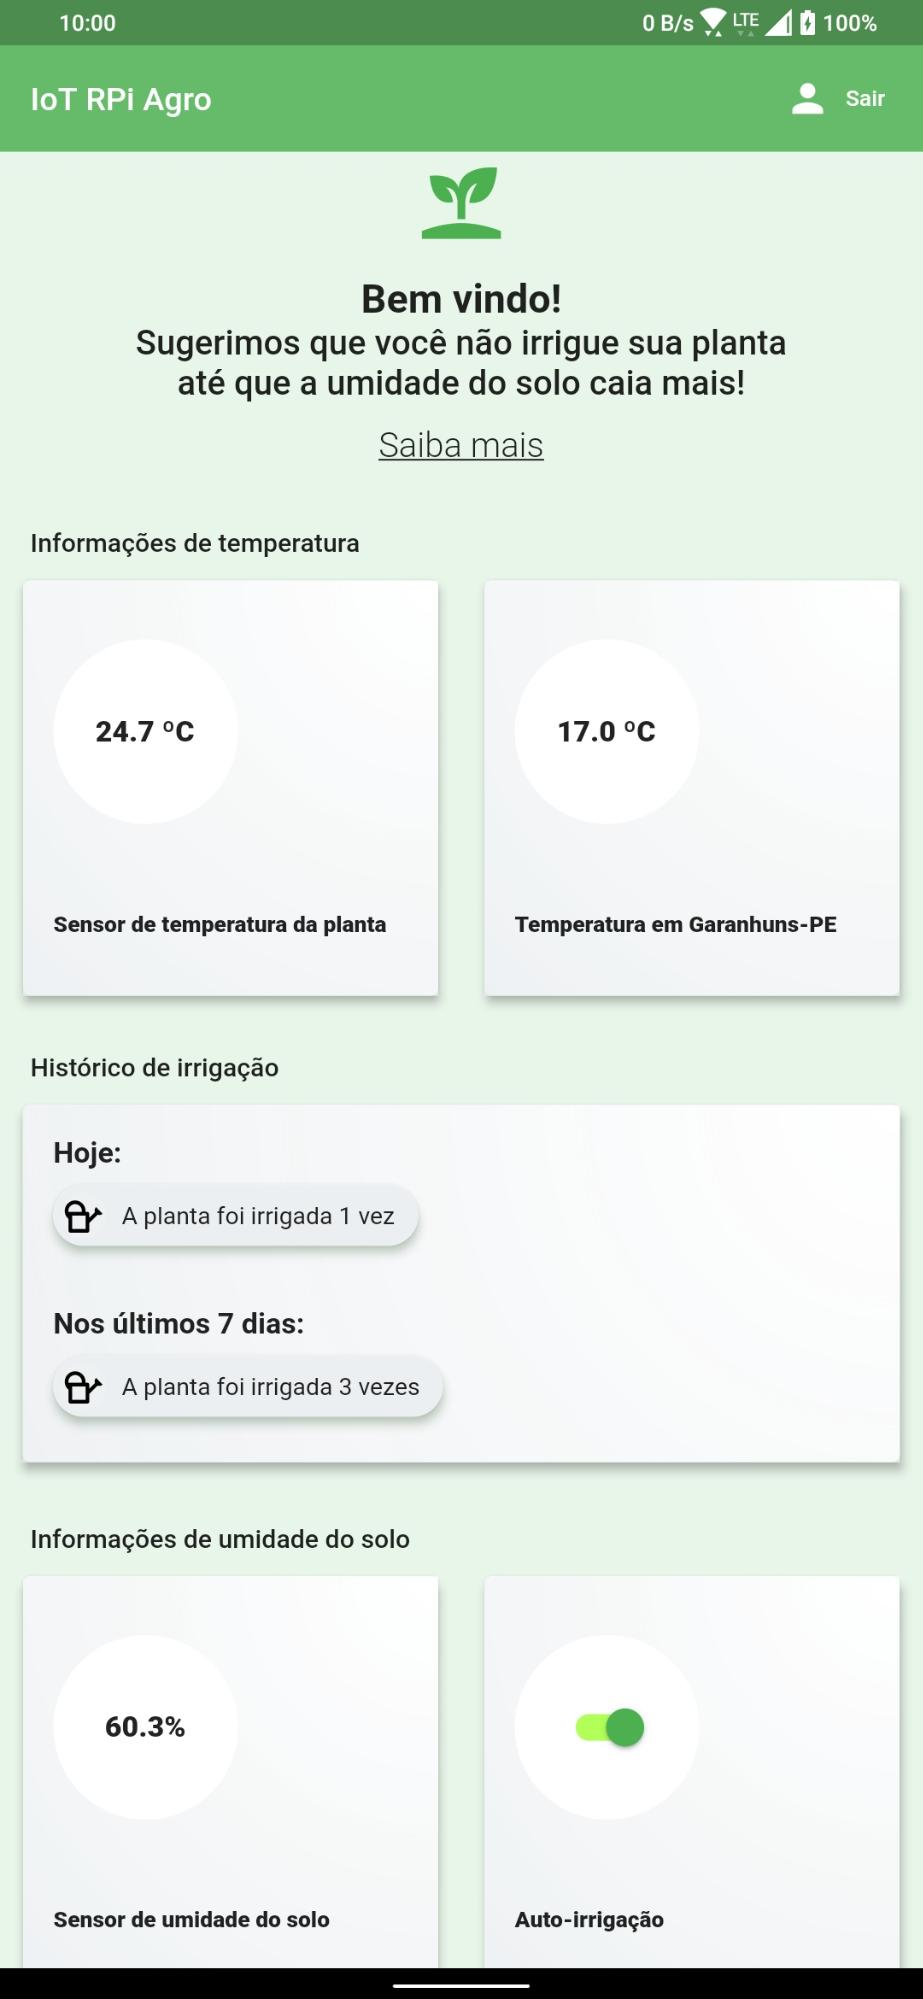
\includegraphics[scale=.25]{Figuras/figura-viii.jpg}}
\caption{Figura VIII}\label{fig-viii}
\end{figure}

\begin{figure}[htbp]
\centerline{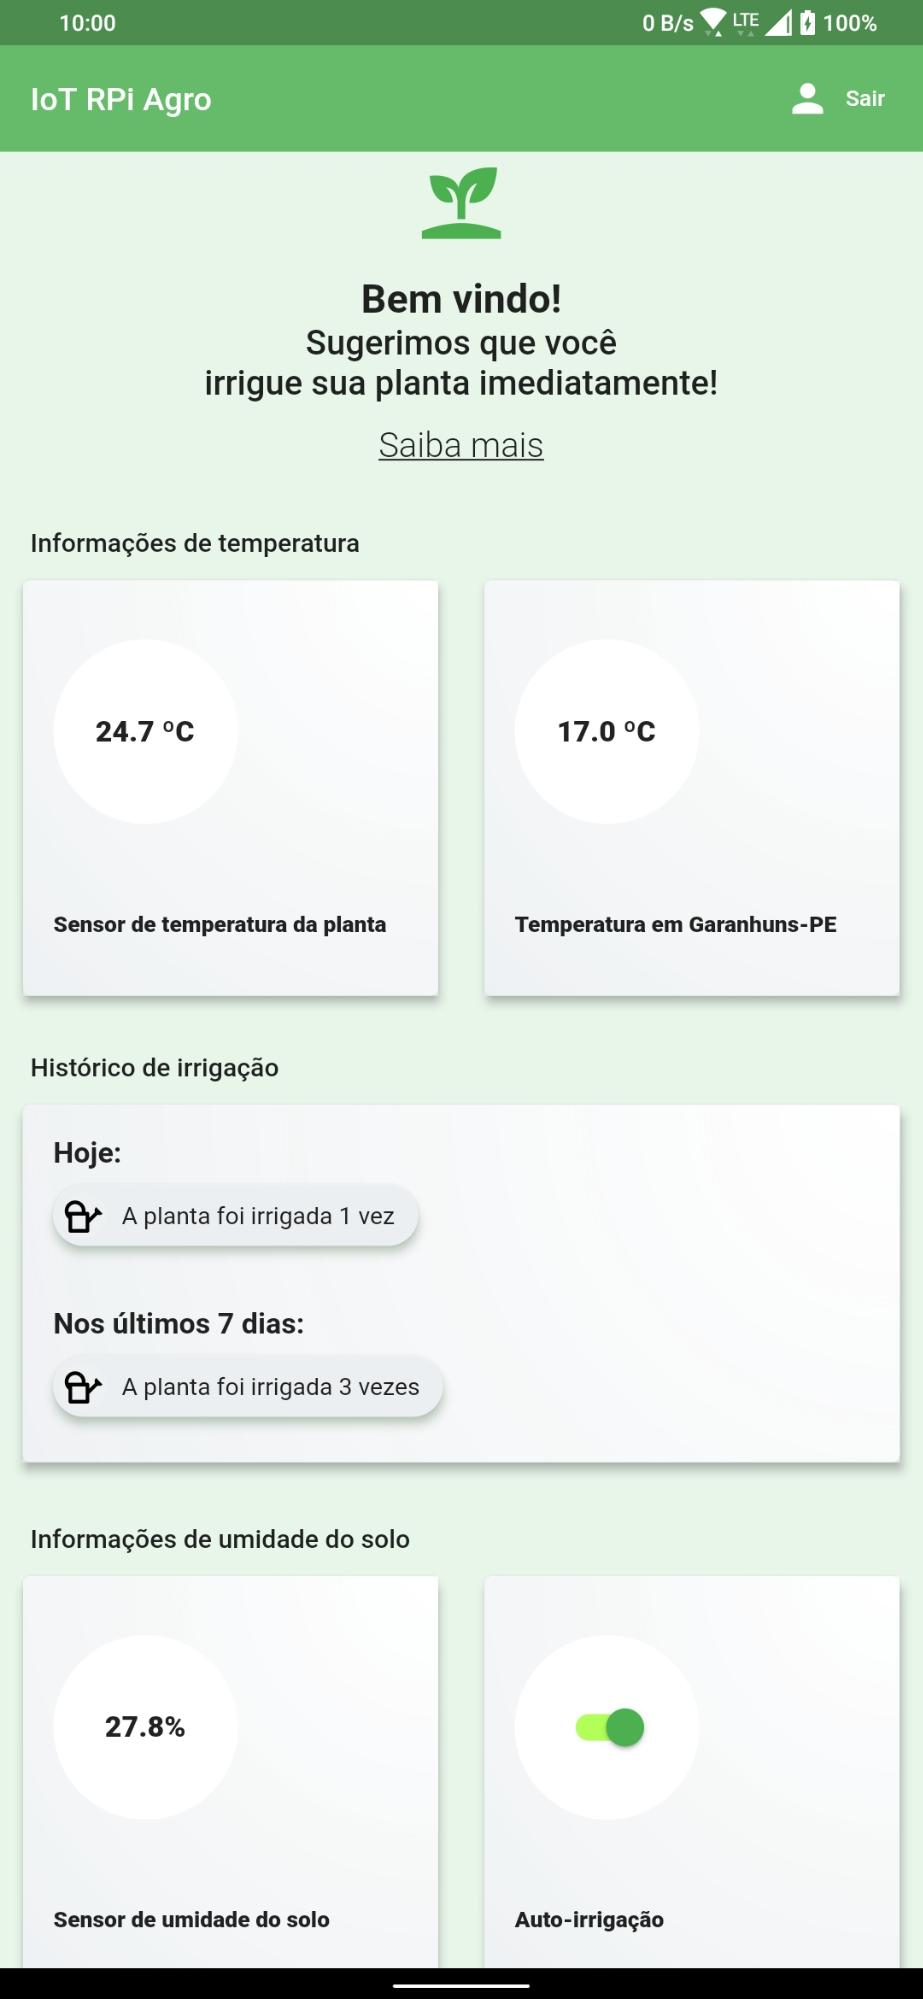
\includegraphics[scale=.25]{Figuras/figura-ix.jpg}}
\caption{Figura IX}\label{fig-ix}
\end{figure}

\chapter{Considerações Finais}\label{chap:consideracoes}

\avisoPIC{}

Esta pesquisa tinha como objetivo avaliar, entender e solucionar lacunas encontradas 
no agronegócio com aplicações em Internet das Coisas, até agora, pude entender como está 
o estado dos estudos e implementações da IoT com a chegada da Indústria 4.0. Em como está 
em crescente desenvolvimento este meio. E como pode-se ter diferentes soluções para vários 
problemas específicos no meio agroeconômico.

Todas as etapas do cronograma foram concluídas, o desenvolvimento da aplicação foi executado 
com sucesso, permitindo assim analisar as novas possibilidades geradas pela Internet das Coisas 
para o agronegócio.


\nocite{*} % Ignore citations (remove if have any)
\bibliographystyle{estilo_ABNT}
\bibliography{refs}
\addcontentsline{toc}{chapter}{Referências Bibliográficas}

% \appendix
% \chapter{Apêndice}\label{ane:relatorio}
% Este é o Apêndice.

\end{document}

